\documentclass{article}
\usepackage[utf8]{inputenc}
\usepackage{hyperref}
\usepackage{graphicx}
\graphicspath{ {images/} }

\hypersetup{
    colorlinks=true,
    linkcolor=blue,
    filecolor=magenta,
    urlcolor=cyan,
    citecolor=black,
}

\title{
MIMBCD-UI
\\
User Testing Guide
}

\author{
  Francisco Maria Calisto\\
  \texttt{francisco.calisto@tecnico.ulisboa.pt}
}

\date{July 2017}

\date{09/04/2018}

\begin{document}

\maketitle

\textbf{Prototype:} \hyperlink{https://github.com/MIMBCD-UI/prototype-breast-cancer}{prototype-breast-cancer} \hfill \textbf{Version:} \hyperlink{https://github.com/MIMBCD-UI/prototype-breast-screening/tree/d88150f25a70153444d185c5eb6c6e99f9b6108a}{v1.0.6-alpha}

\textbf{Milestone:} \hyperlink{https://github.com/MIMBCD-UI/prototype-breast-screening/milestone/6}{1.0.6-alpha} \hfill \textbf{Release:} \hyperlink{https://github.com/MIMBCD-UI/prototype-breast-screening/releases/tag/v1.0.6-alpha}{v1.0.6-alpha}

\hfill

\textbf{DICOM:} \hyperlink{https://github.com/MIMBCD-UI/dicom-server}{dicom-server}

\textbf{Commit:} \hyperlink{https://github.com/MIMBCD-UI/dicom-server/tree/d889ba07d715a3f47bc01634f2163af30b147a20}{d889ba07d715a3f47bc01634f2163af30b147a20}

\hfill

\textbf{Deployment Environment:} Test \hfill \textbf{Deployment Server:} Test

\textbf{Link:} \hyperlink{breastscreening.isr.tecnico.ulisboa.pt}{breastscreening.isr.tecnico.ulisboa.pt}

\hfill

\textbf{Main Server:} \hyperlink{http://breastscreening.isr.tecnico.ulisboa.pt:8081/src/public/index.html}{Test} \hfill \textbf{Port:} 8081

\textbf{Private IP:} \hyperlink{http://10.0.1.23:8081/src/public/index.html}{10.0.1.23} \hfill \textbf{Public IP:} \hyperlink{http://193.136.138.62:8081/src/public/index.html}{193.136.138.62}

\textbf{Private Domain:} \hyperlink{http://cromo.isrnet:8081/src/public/index.html}{cromo.isrnet}

\hfill

\textbf{DICOM Server:} \hyperlink{http://breastscreening.isr.tecnico.ulisboa.pt:8043/app/explorer.html}{Test} \hfill \textbf{Port:} 8043

\textbf{Private IP:} \hyperlink{http://10.0.1.23:8043/app/explorer.html}{10.0.1.23} \hfill \textbf{Public IP:} \hyperlink{http://193.136.138.62:8043/app/explorer.html}{193.136.138.62}

\textbf{Private Domain:} \hyperlink{http://cromo.isrnet:8043/app/explorer.html}{cromo.isrnet} \hfill \textbf{From:} 8143

\clearpage

%%%%%%%%%%%%%%%%%%%%%%%%%%%%%%%%%%%%%%%%%%%%%%%%%%%
%                                                 %
%                     SECTION                     %
%                                                 %
%%%%%%%%%%%%%%%%%%%%%%%%%%%%%%%%%%%%%%%%%%%%%%%%%%%

\section{Introduction}

This document aims to describe the protocol performing a set of tests in the scope of \hyperlink{https://github.com/MIMBCD-UI/prototype-breast-screening/releases/tag/v1.2.0-beta}{v1.2.0-beta} version from the \hyperlink{https://github.com/MIMBCD-UI/prototype-breast-cancer}{prototype-breast-cancer} repository of the \hyperlink{https://mimbcd-ui.github.io/}{MIMBCD-UI} project using traditional devices (mouse and keyboard). The goal of the test is to understand the user, performance, efficiency and efficacy metrics. With the session, the sessions will be recorded via video on the computer and using a record, heat-map and triggered event tools. It is guaranteed the confidentiality of the recordings, which will be used only for academic purposes.

Dividing the activity session into four distinct phases per each two activities representing two different scenarios (Single-Modality vs Multi-Modality). Each scenario will have three patients. In both two scenarios, by supporting our traditional devices, the interaction is made with mouse and keyboard. The first phase, is the \hyperlink{https://docs.google.com/forms/d/1cGmaCGZjeLJhUl_My2wxJ7gcpm7vQRxYhds6Ys0NoSc/edit?usp=sharing}{demographic questionnaire}, where we characterise the Radiologist profile. The second phase is the act of classifying those patients. Radiologists will classify each patient by using the \hyperlink{https://en.wikipedia.org/wiki/BI-RADS}{BIRADS} \cite{balleyguier2007birads}. On the third phase, we will do a small questionnaire at the end of each scenario using \hyperlink{https://en.wikipedia.org/wiki/NASA-TLX}{NASA-TLX}~\cite{ramkumar2017using}. Finally, the forth phase we will have a final survey regarding the Usability of each scenario. The well-known scale called \hyperlink{https, therefore, support this phase://en.wikipedia.org/wiki/System_usability_scale}{System Usability Scale (SUS)}~\cite{orfanou2015perceived}. For the user tests we used a two distinct prototype repositories \hyperlink{https://github.com/MIMBCD-UI/prototype-single-modality}{prototype-single-modality} and \hyperlink{https://github.com/MIMBCD-UI/prototype-multi-modality}{prototype-multi-modality}, both are "almost" mirrors of the \hyperlink{https://github.com/MIMBCD-UI/prototype-breast-cancer}{prototype-breast-cancer} with minor changes.
\section{Material}

At vero eos et accusamus et iusto odio dignissimos ducimus \cite{gardner2008five} qui blanditiis praesentium voluptatum deleniti atque corrupti quos dolores et quas molestias excepturi sint occaecati cupiditate non provident, similique sunt in culpa qui officia deserunt mollitia animi, id est laborum et dolorum fuga.

The material used in the test sessions for the user interface consists of:

\begin{itemize}
  \item Material 1: et harum quidem rerum facilis est et expedita distinctio;
  \item Material 2: et harum quidem rerum facilis est et expedita distinctio;
  \item Material 3: et harum quidem rerum facilis est et expedita distinctio;
  \item Material 4: et harum quidem rerum facilis est et expedita distinctio;
  \item Material 5: et harum quidem rerum facilis est et expedita distinctio;
  \item Material 6: et harum quidem rerum facilis est et expedita distinctio;
  \item Material 7: et harum quidem rerum facilis est et expedita distinctio;
  \item Material 8: et harum quidem rerum facilis est et expedita distinctio;
  \item Material 9: et harum quidem rerum facilis est et expedita distinctio;
\end{itemize}

\clearpage
%%%%%%%%%%%%%%%%%%%%%%%%%%%%%%%%%%%%%%%%%%%%%%%%%%%
%                                                 %
%                     SECTION                     %
%                                                 %
%%%%%%%%%%%%%%%%%%%%%%%%%%%%%%%%%%%%%%%%%%%%%%%%%%%

\section{Description}

To verify our work, we identified measurable and explicit targets. By having several goals, including that a value percentage of the users should be able to operate the tasks without the need of help. On the same rate value, the user should be able to start and complete the medical diagnosis tasks over the system with little errors or mitigating those errors. Measuring the expected number of errors with a relation between our laboratory pilot tests. On the laboratory pilot tests we aim to test our prototypes with Researchers. The Researchers are in the context of the system and know well the functionalities so that we need to expect a percentage value over their results compared to Clinicians and not the same benefits. Last but now least, both users (Researchers and Clinicians) should be able to understand in a similar time amount the meaning of all visible controls. By the similar amount of time, it is expected to have a variance of the percentage value between Researchers and Clinicians of the same value percentage of the early goals described in this paragraph.

We tested each objective in early laboratory and field tests so that we could take the appropriate corrective actions. Also, we expect to run early field tests with Researchers and Clinicians to highlight issues that we overlooked and ignored during the prototyping phase. To support interaction use by the Clinicians, we will try to emphasise several key factors on our user tests. The tasks must be simple, low intrusive, support for natural interaction and the system must always give visibility and the task current-state.

\clearpage

%%%%%%%%%%%%%%%%%%%%%%%%%%%%%%%%%%%%%%%%%%%%%%%%%%%
%                                                 %
%                     SECTION                     %
%                                                 %
%%%%%%%%%%%%%%%%%%%%%%%%%%%%%%%%%%%%%%%%%%%%%%%%%%%

\subsection{Devices}

Traditional interaction remains the most common way to interact with user interfaces in a clinical environment. Unfortunately, most of this interaction is made by low profile equipment that makes users produce more errors and take more time interacting with those user interfaces.

On Figure \ref{fig:patient_list} the user can select the list of patients. The list has a table with several patient information. The first column is the \textit{Patient ID}; we used it as an identifier of the patient. That way we can have anonymised information with no reference to the patient name. The second column is the \textit{Study Date}, the third column is the \textit{Modality} of the used \textbf{DICOM} image, the fourth column is the \textit{Study Description} of the used study and the last column is the number of \textit{Images}.

%%%%%%%%%%%%%%%%%%%%%%%%%%%%%%%%%%%%%%%%%%%%%%%%%%%

\hfill

\begin{figure}[h]
\centering
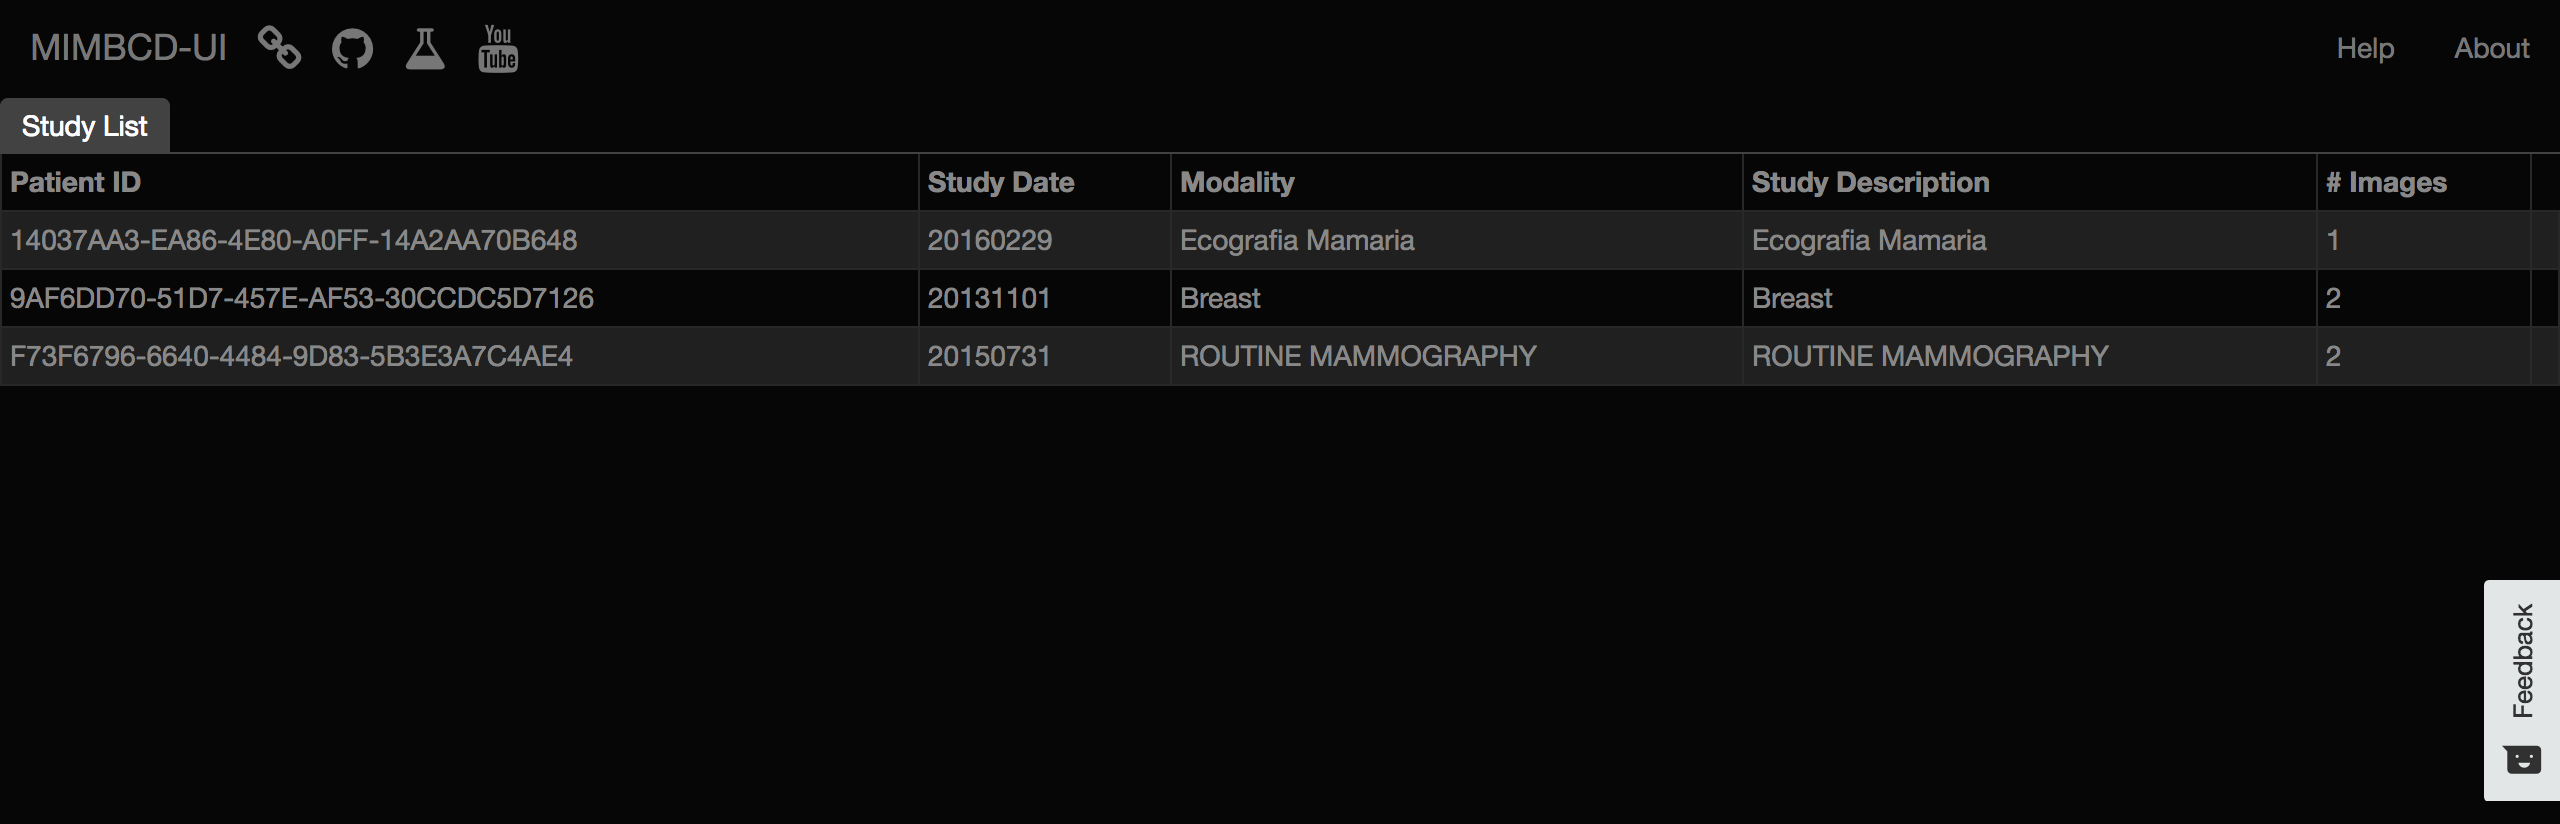
\includegraphics[width=\textwidth]{patient_list}
\caption{List of patients.}
\label{fig:patient_list}
\end{figure}

\hfill

%%%%%%%%%%%%%%%%%%%%%%%%%%%%%%%%%%%%%%%%%%%%%%%%%%%

As we can see in Figure \ref{fig:image_viewer}, it shows the first task in our User Interface (UI), where the patient's breasts are on a small left column. The options are in a short row near of the viewport and described below. We also have the tabs where the user can change the patient. The centre viewport shows the \textbf{DICOM} image, and it can be configured to display a number up to four \textbf{DICOM} images at the same time. The viewport has some text information on it (yellow) with the details of the metadata.

\clearpage

%%%%%%%%%%%%%%%%%%%%%%%%%%%%%%%%%%%%%%%%%%%%%%%%%%%

\hfill

\begin{figure}[h]
\centering
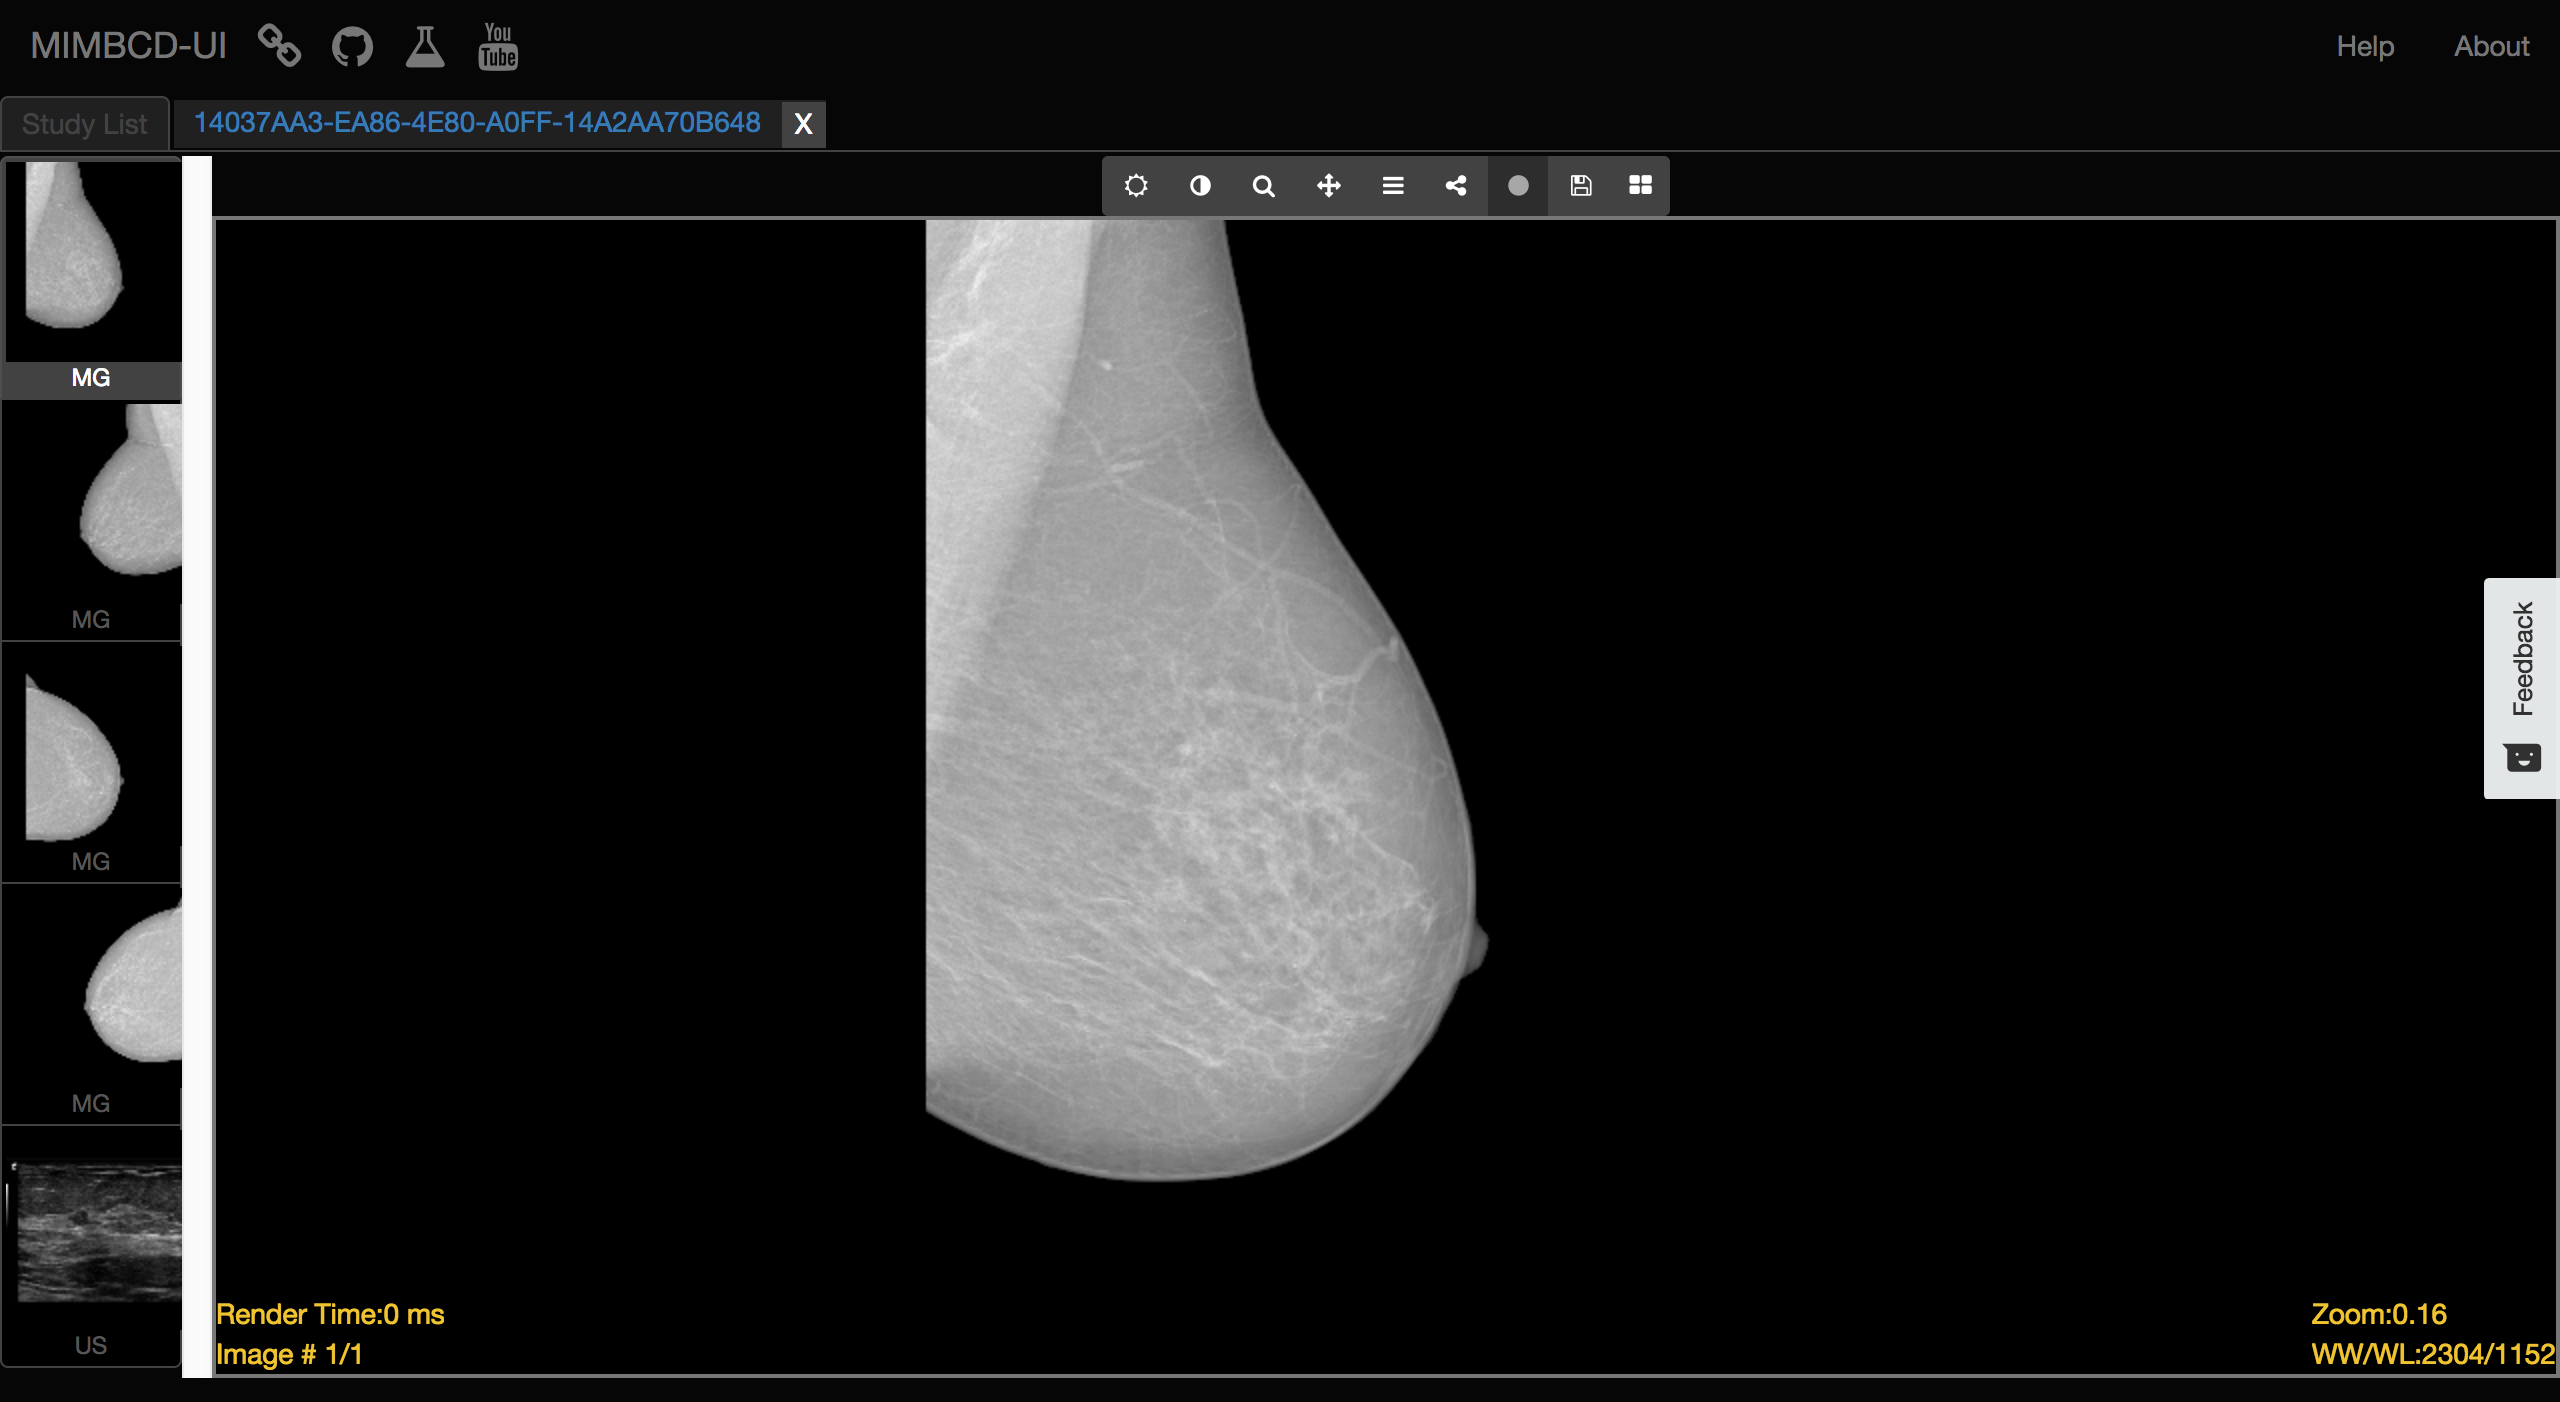
\includegraphics[width=\textwidth]{image_viewer}
\caption{Viewer of the \textbf{DICOM} images.}
\label{fig:image_viewer}
\end{figure}

\hfill

%%%%%%%%%%%%%%%%%%%%%%%%%%%%%%%%%%%%%%%%%%%%%%%%%%%

Manual annotation is adopted by us thanks to Freehand ROI and Probe annotation features, both from CornerstoneJS. According to the CornerstoneJS Library, the user can create an annotation by setting up consecutive landmarks around a Region of Interest (ROI). The markers finish a lesion annotation when it interconnects the historical. Additional features available in our User Interface (UI) includes on-demand increment of the number of landmarks, and throw transformations of the shape of an annotation.

\clearpage

%%%%%%%%%%%%%%%%%%%%%%%%%%%%%%%%%%%%%%%%%%%%%%%%%%%
%                                                 %
%                     SECTION                     %
%                                                 %
%%%%%%%%%%%%%%%%%%%%%%%%%%%%%%%%%%%%%%%%%%%%%%%%%%%

\subsection{User Interactions}

The systems have several buttons (Figure \ref{fig:toolbar}) that allows the user to interact or access to a set of user interface features. Each item of the following list represents each metaphoric icon of Figure \ref{fig:toolbar}.

%%%%%%%%%%%%%%%%%%%%%%%%%%%%%%%%%%%%%%%%%%%%%%%%%%%

\hfill

\begin{figure}[h]
\centering

\includegraphics[width=\textwidth]{toolbar}
\caption{Toolbar of the System available features.}
\label{fig:toolbar}
\end{figure}

\hfill

%%%%%%%%%%%%%%%%%%%%%%%%%%%%%%%%%%%%%%%%%%%%%%%%%%%

\hfill

The buttons are (from left to right of Figure \ref{fig:toolbar}) as follows:

\hfill

\begin{itemize}
\item WW/WC
\item Invert
\item Zoom
\item Pan
\item Stack Scroll
\item Freehand
\item Probe
\item Save
\item Window Controller
\end{itemize}

\hfill

\clearpage

%%%%%%%%%%%%%%%%%%%%%%%%%%%%%%%%%%%%%%%%%%%%%%%%%%%
%                                                 %
%                     SECTION                     %
%                                                 %
%%%%%%%%%%%%%%%%%%%%%%%%%%%%%%%%%%%%%%%%%%%%%%%%%%%

\subsection{Usability Evaluation Technique}

Usability and functionality are the significant elements which can significantly affect the performance of a medical system. While some prior studies \cite{Calisto:2017:TTM:3132272.3134111} have investigated the functionality of healthcare systems, the usability issue has mostly been overlooked in the existing Health Informatics (HI) literature regarding Human-Computer Interaction (HCI).

The following Table \ref{table:key_questions} is presenting six evaluation questions to have in mind during evaluation. The purpose of this questions is to facilitate systematic user studies in a clinical environment and support the identification of usability problems. The proposed issues involve various aspects of workload combined with either need for satisfaction or division of attention.

\begin{table}[h]
\centering
\label{table:key_questions}
\begin{tabular}{l|l}
Number & Issues of Content Key Questions                    \\ \hline
1      & How do you perceive this activity?                 \\
2      & Could it be done in a more intuitive way?          \\
3      & What are the consequences?                         \\
4      & Why did you do as you did with this activity?      \\
5      & Is this activity relevant for you?                 \\
6      & Could you suggest another way to do this activity?
\end{tabular}
\caption{Usability Evaluation Questions}
\end{table}

The influence of perceived activity \cite{flavian2006role} is an important variable for our empirical analysis. In fact, the trust of the user increases when the user perceived that the system is usable and that there will be a consequent increase of the clinician trust in our system. This arguments explains the first question, the \textit{How do you perceive this activity?} question. For the second question, the \textit{Could it be done in a more intuitive way?} question, we aim to conclude if there is some solution for a more intuitive way of perceive the activity. Third, we intend to filter possible consequences of the clinician workflow by asking \textit{What are the consequences?} directly to the clinician. The fourth question, underlines the reasons why the clinician did that way, with the question \textit{Why did you do as you did with this activity?} we can understand the process of achieving the activity goal and the clinician's interpretation of it. On the fifth question, where we ask \textit{Is this activity relevant for you?}, we aim to understand the potential relevance of our system to the clinician. Last but not least, the six question is present to give the clinician opportunity to suggest improvements, reflecting the reasons why we ask the \textit{Could you suggest another way to do this activity?} question.

To conclude this section, by doing this questions, we aim to support our user studies by giving our users, the clinicians, the opportunity of improving our empirical analysis regarding user's \textit{open answers}. However, the results should be treated with caution. Several bias exists since we are doing here an ambiguous approach.

\clearpage
\section{System}

Lorem ipsum dolor sit amet, consectetur adipiscing elit, sed do eiusmod tempor incididunt ut labore et dolore magna aliqua. Ut enim ad minim veniam, quis nostrud exercitation ullamco laboris nisi ut aliquip ex ea commodo consequat. Duis aute irure dolor in reprehenderit in voluptate velit esse cillum dolore eu fugiat nulla pariatur. Excepteur sint occaecat cupidatat non proident, sunt in culpa qui officia deserunt mollit anim id est laborum.

%%%%%%%%%%%%%%%%%%%%%%%%%%%%%%%%%%%%%%%%%%%%%%%%%%%
%                                                 %
%                     SECTION                     %
%                                                 %
%%%%%%%%%%%%%%%%%%%%%%%%%%%%%%%%%%%%%%%%%%%%%%%%%%%

\subsection{Environments}

Lorem ipsum dolor sit amet, consectetur adipiscing elit, sed do eiusmod tempor incididunt ut labore et dolore magna aliqua. Ut enim ad minim veniam, quis nostrud exercitation ullamco laboris nisi ut aliquip ex ea commodo consequat. Duis aute irure dolor in reprehenderit in voluptate velit esse cillum dolore eu fugiat nulla pariatur. Excepteur sint occaecat cupidatat non proident, sunt in culpa qui officia deserunt mollit anim id est laborum.

%%%%%%%%%%%%%%%%%%%%%%%%%%%%%%%%%%%%%%%%%%%%%%%%%%%

\hfill

%\begin{figure}[h]
%\caption{Image Sample}
%\centering
%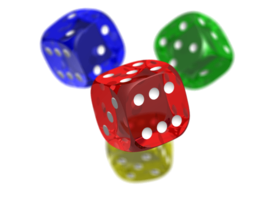
\includegraphics[width=\textwidth]{image}
%\end{figure}

\hfill

%%%%%%%%%%%%%%%%%%%%%%%%%%%%%%%%%%%%%%%%%%%%%%%%%%%

Nisi ut aliquid ex ea commodi consequatur? Vel illum qui dolorem eum fugiat quo voluptas nulla pariatur?

%%%%%%%%%%%%%%%%%%%%%%%%%%%%%%%%%%%%%%%%%%%%%%%%%%%
%                                                 %
%                     SECTION                     %
%                                                 %
%%%%%%%%%%%%%%%%%%%%%%%%%%%%%%%%%%%%%%%%%%%%%%%%%%%

\subsection{Interaction}

Lorem ipsum dolor sit amet, consectetur adipiscing elit, sed do eiusmod tempor incididunt ut labore et dolore magna aliqua. Ut enim ad minim veniam, quis nostrud exercitation ullamco laboris nisi ut aliquip ex ea commodo consequat. Duis aute irure dolor in reprehenderit in voluptate velit esse cillum dolore eu fugiat nulla pariatur. Excepteur sint occaecat cupidatat non proident, sunt in culpa qui officia deserunt mollit anim id est laborum.

%%%%%%%%%%%%%%%%%%%%%%%%%%%%%%%%%%%%%%%%%%%%%%%%%%%

\hfill

%\begin{figure}[h]
%\caption{Banner Sample}
%\centering
%
\includegraphics[width=\textwidth]{banner}
%\end{figure}

\hfill

%%%%%%%%%%%%%%%%%%%%%%%%%%%%%%%%%%%%%%%%%%%%%%%%%%%

\hfill

List of something with no enumeration:

\hfill

\begin{itemize}
  \item Something 1
  \item Something 2
  \item Something 3
  \item Something 4
  \item Something 5
  \item Something 6
  \item Something 7
  \item Something 8
  \item Something 9
\end{itemize}

\hfill

%%%%%%%%%%%%%%%%%%%%%%%%%%%%%%%%%%%%%%%%%%%%%%%%%%%

Lorem ipsum dolor sit amet, consectetur adipiscing elit, sed do eiusmod tempor incididunt ut labore et dolore magna aliqua. Ut enim ad minim veniam, quis nostrud exercitation ullamco laboris nisi ut aliquip ex ea commodo consequat. Duis aute irure dolor in reprehenderit in voluptate velit esse cillum dolore eu fugiat nulla pariatur.
\section{Procedures}

Participants will take part in the tests at the \hyperlink{http://hff.min-saude.pt/}{Hospital Fernando Fonseca (HFF)} with the \hyperlink{https://github.com/MIMBCD-UI/prototype-breast-screening/releases/tag/v1.0.6-alpha}{v1.0.6-alpha} version of our \hyperlink{https://github.com/MIMBCD-UI/prototype-breast-screening/}{prototype-breast-screening}. The interaction with the system will be used in a typical \textbf{RR} environment. Note takers and data logger(s) will monitor the sessions for observation in the \textbf{RR}, connected by screen recording feed. The test sessions will be recorded and further analysed.

%%%%%%%%%%%%%%%%%%%%%%%%%%%%%%%%%%%%%%%%%%%%%%%%%%%
%                                                 %
%                     SECTION                     %
%                                                 %
%%%%%%%%%%%%%%%%%%%%%%%%%%%%%%%%%%%%%%%%%%%%%%%%%%%

\subsection{Briefing}

A presentation of the systems and it's use and capabilities will be made. Participants will be presented to the available interactions and will be explained how to interact with the prototype, underlining the limitations. The facilitator will brief the participants on the prototype application and instruct the participant that they are evaluating the application, rather than the facilitator evaluating the participant. Participants will sign an informed consent that acknowledges: the participation is voluntary, that participation can cease at any time, and that the session will be videotaped but their privacy of identification will be granted. The facilitator will ask the participant if they have any question.

%%%%%%%%%%%%%%%%%%%%%%%%%%%%%%%%%%%%%%%%%%%%%%%%%%%

%%%%%%%%%%%%%%%%%%%%%%%%%%%%%%%%%%%%%%%%%%%%%%%%%%%
%                                                 %
%                     SECTION                     %
%                                                 %
%%%%%%%%%%%%%%%%%%%%%%%%%%%%%%%%%%%%%%%%%%%%%%%%%%%

\subsection{Post-Task Questionnaire}

Our metrics will refer the user performance measured against specific performance goals necessary to satisfy several requirements of our system. For our \textbf{Post-Task Questionnaire} we will use \textbf{SUS} to measure the usability of our system each time a \textit{task} is completed. From a set of tasks (see \textbf{Tasks} section) we aim to cover several scenarios. Therefore, the \textbf{SUS} will allow the facilitator to quickly and easily assess the usability of a given scenario. This scale has several attributes \cite{bangor2008empirical} that make it a good choice for our clinical usability participants. Those attributes are as follows.

\hfill

%%%%%%%%%%%%%%%%%%%%%%%%%%%%%%%%%%%%%%%%%%%%%%%%%%%

List of the scale attributes:

%%%%%%%%%%%%%%%%%%%%%%%%%%%%%%%%%%%%%%%%%%%%%%%%%%%

\hfill

\begin{itemize}
  \item The survey is technology agnostic, making it flexible enough;
  \item The survey is relatively quick and easy to use;
  \item The survey provides a single score on a scale that is easily understood;
  \item The survey is nonproprietary, making it a cost effective tool;
\end{itemize}

\hfill

%%%%%%%%%%%%%%%%%%%%%%%%%%%%%%%%%%%%%%%%%%%%%%%%%%%

The facilitator will explain that the amount of time taken to complete the \textit{tasks} will be measured and that exploratory behaviour outside the \textit{task} flow should not occur until after task completion. At the beginning of each task, the participant will listen the task description from the facilitator and begin the task. \textit{Time-on-task} measurements begins when the participant starts the \textit{task}, measured until the end of each \textit{task}.

%%%%%%%%%%%%%%%%%%%%%%%%%%%%%%%%%%%%%%%%%%%%%%%%%%%

%%%%%%%%%%%%%%%%%%%%%%%%%%%%%%%%%%%%%%%%%%%%%%%%%%%
%                                                 %
%                     SECTION                     %
%                                                 %
%%%%%%%%%%%%%%%%%%%%%%%%%%%%%%%%%%%%%%%%%%%%%%%%%%%

\subsection{Training Session}

The participant will receive and overview the usability test procedure. However, the user will not receive information how to annotate and interact in all degrees of freedom. With the aim of disabling users to get their work done before the test tasks. It will take advantage of a "surprise" acknowledgement.

%%%%%%%%%%%%%%%%%%%%%%%%%%%%%%%%%%%%%%%%%%%%%%%%%%%
%                                                 %
%                     SECTION                     %
%                                                 %
%%%%%%%%%%%%%%%%%%%%%%%%%%%%%%%%%%%%%%%%%%%%%%%%%%%

\subsection{Execution of Tasks}

The \textit{tasks} were derived from test scenarios developed from \textbf{Case Studies}. Due to the range and extent of functionality provided by our prototype, and the short time from which each participant will be available, the \textit{tasks} are the most common and relatively complex of available functions. The \textit{tasks} are the identical for all participants of a given user role in the study.

The \textit{tasks} will be performed by several classes of radiology experience. Professionals from Radiology Seniors, Juniors and Interns will be performing these \textit{tasks}. On the \textbf{RR} the Radiologist is characterised~\cite{ehrlich2016patient, miglioretti2007radiologist} as a physician who examines and interpret Medical Imaging (MI) \cite{kobashi2017evaluation}, such as X-Rays, CT Scans or MRIs.

%%%%%%%%%%%%%%%%%%%%%%%%%%%%%%%%%%%%%%%%%%%%%%%%%%%

%%%%%%%%%%%%%%%%%%%%%%%%%%%%%%%%%%%%%%%%%%%%%%%%%%%
%                                                 %
%                     SECTION                     %
%                                                 %
%%%%%%%%%%%%%%%%%%%%%%%%%%%%%%%%%%%%%%%%%%%%%%%%%%%

\subsection{Post-Activity Questionnaire}

After completing all \textit{tasks} and scenarios, participants will be asked to complete a questionnaire to classify the prototype according to various parameters regarding the workload. To measure this, we will use the well known scale called \hyperlink{https://en.wikipedia.org/wiki/NASA-TLX}{NASA-TLX}~\cite{ramkumar2017using}. It consists of a set of six rating scales to evaluate the workload of the participant in a \textit{task} or a set of \textit{tasks}. \hyperlink{https://en.wikipedia.org/wiki/NASA-TLX}{NASA-TLX} is used in \textbf{Human-Computer Interaction (HCI)} research to identify users' performance, metal demand, emotion, etc. We will use this scale questionnaire to identify participants' workload during the various stages of the workflow.

%%%%%%%%%%%%%%%%%%%%%%%%%%%%%%%%%%%%%%%%%%%%%%%%%%%
\section{Tasks}
\label{sec:sec006}

During our user tests, we need to ask participants to provide a subjective assessment of their experience using our \textbf{Assistant}. There are several widely used questionnaires giving us different prons-and-cons. However, in most cases, a \hyperlink{https://www.nngroup.com/articles/keep-online-surveys-short/}{single question instrument}~\cite{sauro201210} is the right method for a quantitative usability testing. By taking less time and effort to answer, participants are pursuing to this phase after task while it is minimally disruptive.

\clearpage

%%%%%%%%%%%%%%%%%%%%%%%%%%%%%%%%%%%%%%%%%%%%%%%%%%%

\hfill

\begin{wrapfigure}{r}{0.50\textwidth}
\centering
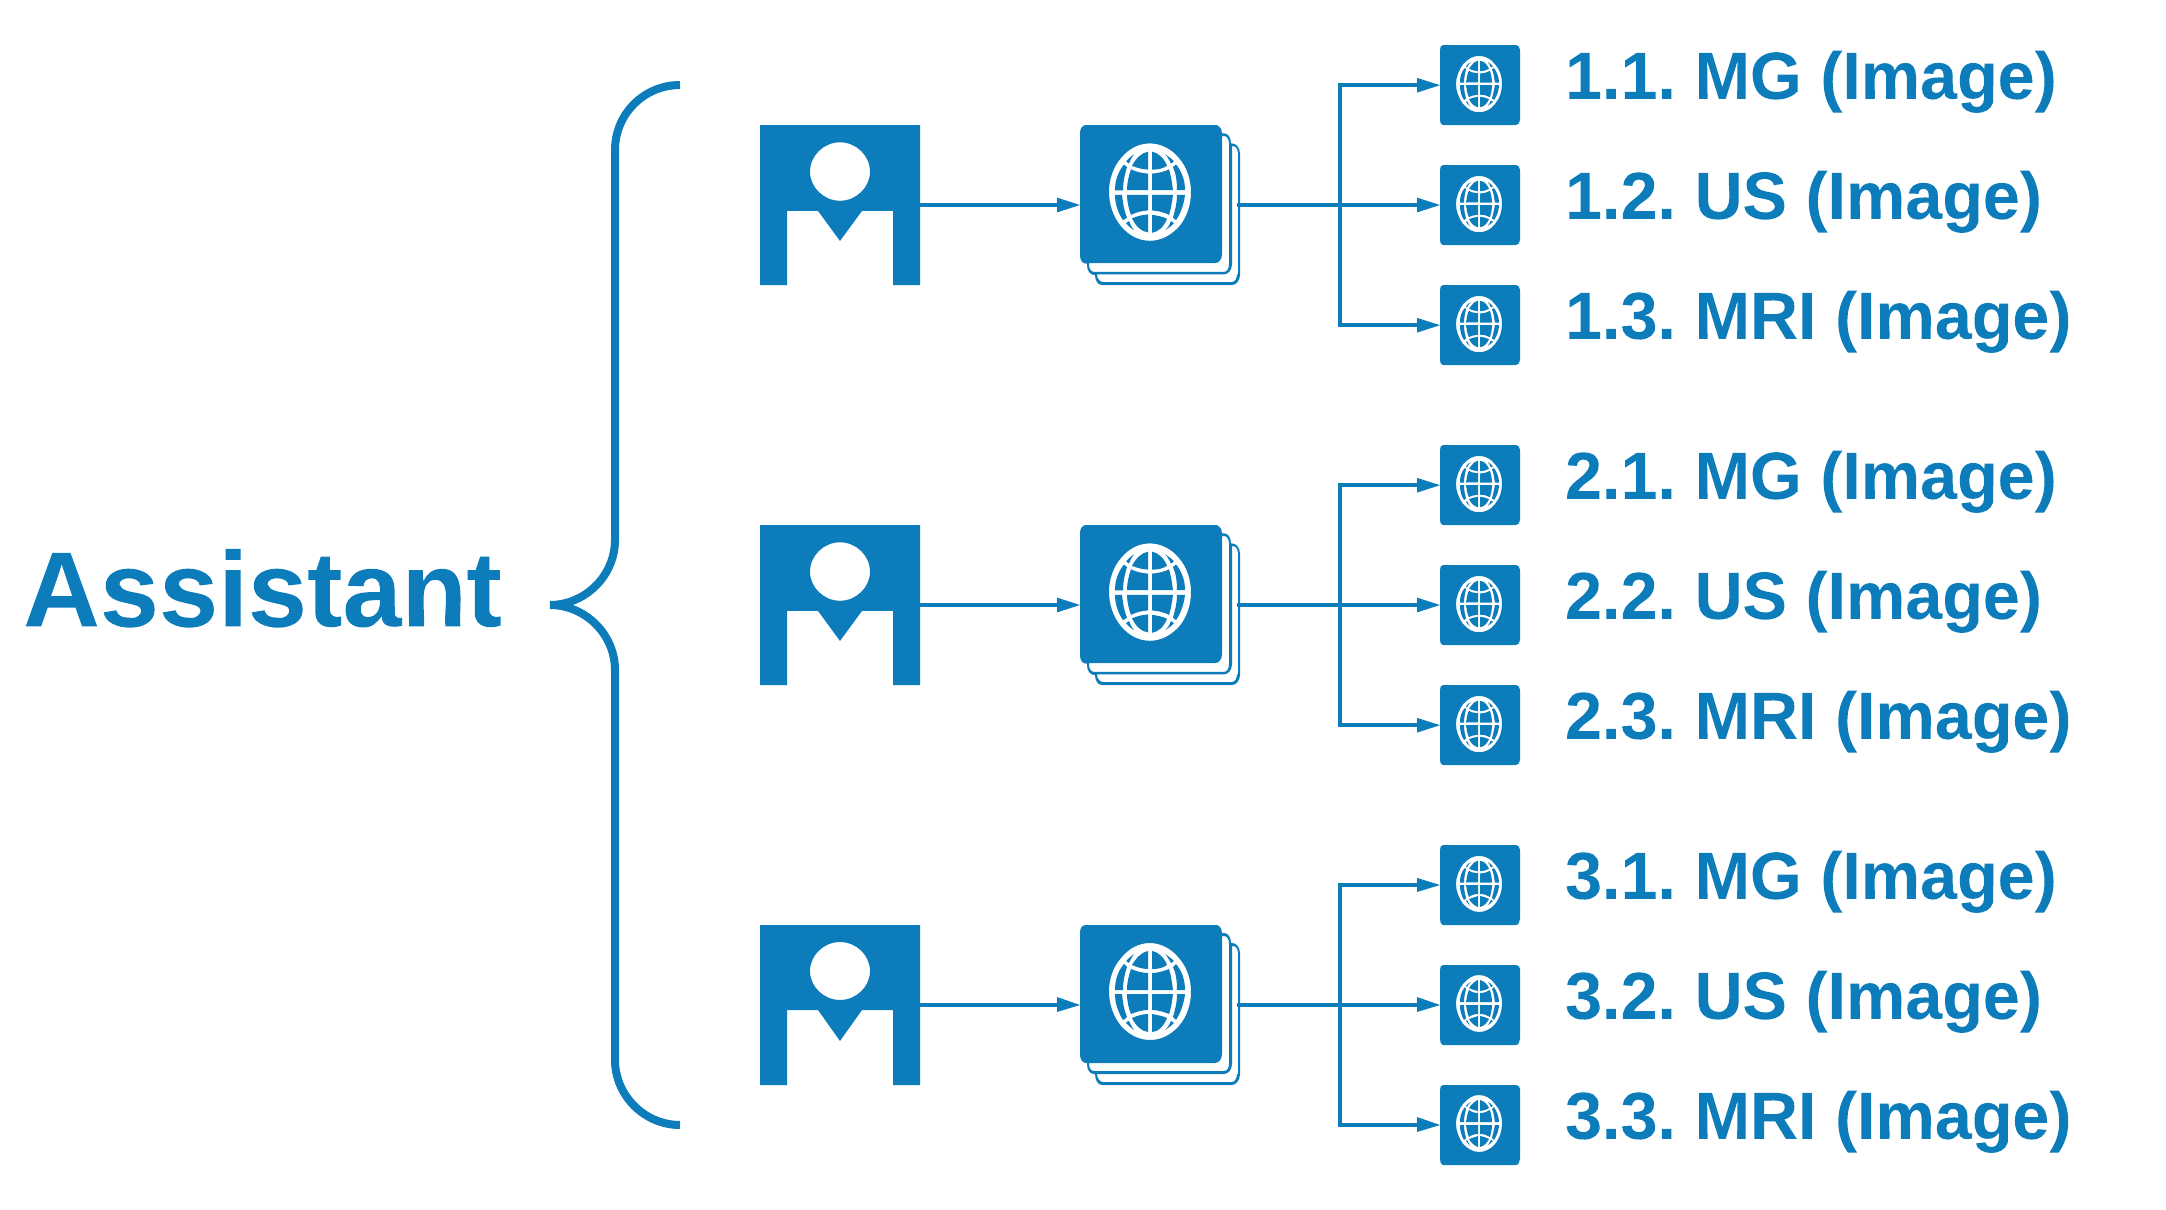
\includegraphics[width=0.50\textwidth]{img001}
\caption{Diagram representing the use of the \textbf{Assistant} by clinicians.}
\label{fig:svmm}
\end{wrapfigure}

\hfill

%%%%%%%%%%%%%%%%%%%%%%%%%%%%%%%%%%%%%%%%%%%%%%%%%%%

We will try to understand if, with the \textit{AI-Assisted} techniques, the clinicians will encounters the most accurate severity (\hyperlink{https://en.wikipedia.org/wiki/BI-RADS}{BIRADS}) of the breast lesions~\cite{american1998breast} and patient's prognostic. For this purpose, we have three patients (Figure \ref{fig:svmm}); each patient has three images in the respective modalities: (i) MG; (ii) US; and (iii) MRI. The clinicians will proceed to the activity of diagnosing the three patients within the support of our \textbf{Assistant} by the observation of ALL images.

\hfill

In our \textbf{User Testing Guide} a set of tasks is necessary and carefully crafted. Our test studies involve asking participants to perform a set of tasks. By looking at what our user need to do with our system, our tasks are realistic as possible. We are not describing the exact steps participants need to take. We achieve that by avoiding the precise language used as labels in our system. The tasks are emotionally neutrals. And we did several \hyperlink{https://www.nngroup.com/articles/pilot-testing/}{pilot tests} to prevent misleading situations saving us from wasting resources by accidentally use a lousy task or from getting bad data. The tasks are as follows.

\hfill

%%%%%%%%%%%%%%%%%%%%%%%%%%%%%%%%%%%%%%%%%%%%%%%%%%%

List of stand alone tasks:

%%%%%%%%%%%%%%%%%%%%%%%%%%%%%%%%%%%%%%%%%%%%%%%%%%%

\hfill

\begin{itemize}
\item[] \textbf{Task 1.1:} Classify \textit{Patient 1} on the \textbf{Assistant};
\item[] \textbf{Task 1.2:} Classify \textit{Patient 2} on the \textbf{Assistant};
\item[] \textbf{Task 1.3:} Classify \textit{Patient 3} on the \textbf{Assistant};
\end{itemize}

\hfill

\begin{itemize}
\item[] \textbf{Task 2.1:} Freely explore \textit{Patient 1} on the \textbf{Assistant};
\item[] \textbf{Task 2.2:} Freely explore \textit{Patient 2} on the \textbf{Assistant};
\item[] \textbf{Task 2.3:} Freely explore \textit{Patient 3} on the \textbf{Assistant};
\end{itemize}

\hfill

%%%%%%%%%%%%%%%%%%%%%%%%%%%%%%%%%%%%%%%%%%%%%%%%%%%

\clearpage
\section{Measurements}

Lorem ipsum dolor sit amet, consectetur adipiscing elit, sed do eiusmod tempor incididunt ut labore et dolore magna aliqua. Ut enim ad minim veniam, quis nostrud exercitation ullamco laboris nisi ut aliquip ex ea commodo consequat. Duis aute irure dolor in reprehenderit in voluptate velit esse cillum dolore eu fugiat nulla pariatur. Excepteur sint occaecat cupidatat non proident, sunt in culpa qui officia deserunt mollit anim id est laborum.

\begin{itemize}
  \item Measurement 1;
  \item Measurement 2;
  \item Measurement 3;
  \item Measurement 4;
  \item Measurement 5;
  \item Measurement 6;
  \item Measurement 7;
  \item Measurement 8;
  \item Measurement 9;
\end{itemize}

Lorem ipsum dolor sit amet, consectetur adipiscing elit, sed do eiusmod tempor incididunt ut labore et dolore magna aliqua. Ut enim ad minim veniam, quis nostrud exercitation ullamco laboris nisi ut aliquip ex ea commodo consequat. Duis aute irure dolor in reprehenderit in voluptate velit esse cillum dolore eu fugiat nulla pariatur. Excepteur sint occaecat cupidatat non proident, sunt in culpa qui officia deserunt mollit anim id est laborum.

\begin{itemize}
  \item Difficulty of ...
  \item Difficulty of ...
  \item Difficulty of ...
  \item Degree of ...
\end{itemize}

\clearpage

\bibliographystyle{plain}
\bibliography{bibliography/references.bib}

\end{document}